
\usetikzlibrary{shapes.geometric}
\usetikzlibrary{positioning}

% =========================================
\begin{block}{Deterministic Protocols and Maximally Hard}

\textbf{Overview.}
Building on the two-party model defined previously, in this section we will formalize
deterministic protocols and maximally hard functions.
We then prove that \textsc{Equality} is deterministically maximally hard
and embed it into \textsc{TRAV} to show that \textsc{TRAV} is also maximally hard.

\vspace{0.6em}

\textbf{Deterministic Protocol.}
A fixed, non-randomness communication procedure that outputs
$f(x,y)$ correctly for every input pair. At each step, the next message is determined solely by the party’s previous input and the transcript so far.


\vspace{0.6em}

\textbf{Maximally Hard.}
A function $f$ is maximally hard if $D(f) = \Theta(n)$

In the worst case, one party can always solve the problem by sending all $n$ of their input bits to the other party. Therefore, linear communication is the largest possible asymptotic complexity. Any function requiring $\Omega(n)$ bits is maximally hard.


\end{block}

% =========================================
\begin{block}{Equality is Deterministically Maximally Hard}

\textbf{Equality Problem: } Do Alice and Bob hold the same $n$-bit string?
\[
\textsc{EQ}(x,y)=
\begin{cases}
1 & x=y \\
0 & x\neq y
\end{cases}
\]\\[30pt]


\begin{columns}[T]

\column{0.65\textwidth}

We visualize $\textsc{EQ}$ using its communication matrix:
rows are Alice’s inputs, columns are Bob’s inputs,
and a dot marks where $\textsc{EQ}(x,y)=1$.\\

\vspace{0.8em}

All 1-outputs lie on the diagonal, since equality holds
iff $x=y$. Every off-diagonal entry is 0.\\

\column{0.30\textwidth}

\begin{center}
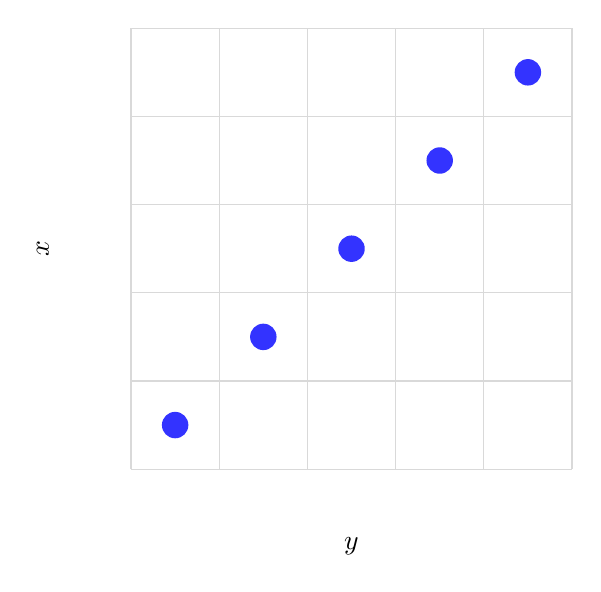
\begin{tikzpicture}[scale=1.4]
\draw[step=0.8cm,gray!30] (0,0) grid (4,4);
\foreach \i in {0.4,1.2,2.0,2.8,3.6}
    \fill[blue!80] (\i,\i) circle (0.12);
\node at (2,-0.7) {\textbf{$y$}};
\node[rotate=90] at (-0.8,2) {\textbf{$x$}};
\end{tikzpicture}
\end{center}

\end{columns}

A deterministic protocol must partitions this matrix into 
\emph{monochromatic rectangles}, meaning submatrices where all entries 
have the same output (all 0’s or all 1’s).

Because the 1’s lie only on the diagonal, no two distinct diagonal entries
can share such a rectangle without including a 0. Thus each diagonal 1 must be isolated.

There are $2^n$ diagonal entries, so $D(\textsc{EQ}) \ge n$. Thus this must mean Equality is maximally hard.

\end{block}
›$$
% =========================================
% =========================================
\begin{block}{Embedding Equality into TRAV}

To prove that \textsc{TRAV} is maximally hard, we reduce 
\textsc{Equality} to \textsc{TRAV}.

\vspace{0.6em}

For each bit position $i$, we construct a gadget that depends on 
Alice’s bit $x_i$ and Bob’s bit $y_i$.

\begin{figure}[H]
\centering
\begin{tikzpicture}[
hex/.style={
draw,
regular polygon,
regular polygon sides=6,
minimum size=5cm,
inner sep=0pt
}
]

\node[hex] (h1) at (0,0)  {\scriptsize $i=1$};
\node[hex] (h2) at (5,0)  {\scriptsize $i=2$};
\node[hex] (h3) at (10,0) {\scriptsize $i=3$};
\node[hex] (h4) at (15,0) {\scriptsize $\cdots$};
\node[hex] (h5) at (20,0) {\scriptsize $i=n$};

\node[above=4pt of h3] {\scriptsize $x_i = y_i = 1$};
\node[below=4pt of h3] {\scriptsize $x_i = y_i = 0$};

\end{tikzpicture}
\caption{Chain of Equality Gadgets}
\end{figure}

In our gadget, the path is only traversable at index $i$ if $x_i$ and $y_i$ are both 0 or 1. In other words each gadget is traversable if and only if $x_i = y_i$.

We connect all gadgets in sequence.  
Therefore, a path exists from the first gadget to the last  
if and only if $x_i = y_i$ for all $i$, i.e., if and only if $x=y$.

\vspace{0.6em}

Thus,
\[
\textsc{EQ} \le \textsc{TRAV}.
\]

Since $\textsc{EQ}$ is deterministically maximally hard,
$\textsc{TRAV}$ must also require $\Omega(n)$ communication.

\textbf{Therefore, TRAV is deterministically maximally hard.}

\end{block}